\documentclass[12pt,a4paper,titlepage,twoside]{book}
\usepackage{chngcntr}
\usepackage[bottom]{footmisc}
\usepackage[applemac]{inputenc}
\usepackage[italian]{babel}
\usepackage{guit}
\usepackage[autostyle, italian=guillemets]{csquotes}
\usepackage[T1]{fontenc}
\usepackage{graphicx}
\usepackage{setspace}
\usepackage{frontespizio}
\usepackage{imakeidx}
\usepackage{midpage}
\makeindex[]
\begin{document}

	\begin{flushleft}
		\large
		\textsc{Giulia Franco} \\
		\textsc{matricola SM3500370}\\
		\textsc{Year 2018/2019}
		\\
		\textsc{Exercise 1,Parallel Computing course.}
	\end{flushleft}
\newpage
\begin{figure}
	\section*{Computing pi using openMP.}
	The aim of the exercise is to compute $\pi$ using midpoints rule. The code is implemented using an openMP approach, exploiting the multithreads computation. In the code (\textit{pi.c}) three different pragma sections:\\
	-\textit{critical}=A thread waits at the start of a critical region until no other thread in the program is executing a critical region with that same name.\\
	-\textit{atomic}=Allows access of a specific memory location atomically to threads. It ensures that race conditions are avoided through direct control of concurrent threads that might read or write to or from the particular memory location.\\
	-\textit{reduction}=Creates a private variable for each thread and finally all the resuts are accumulated using operations.
	\\
	These methods are compared with respect to the serial computation using $"omp\_get\_wtime()"$, using different number of threads.
	\begin{center}
		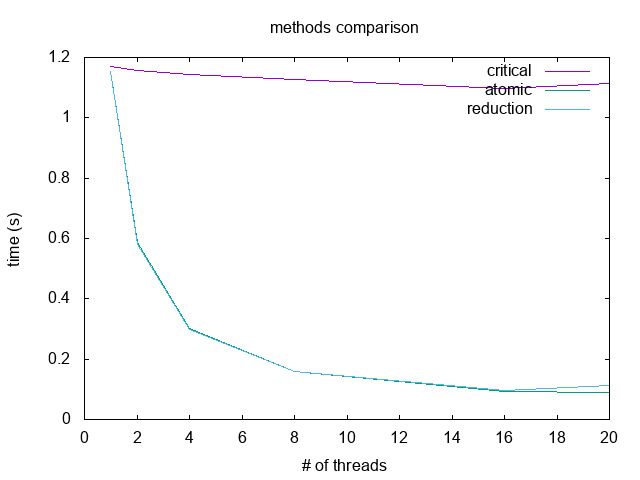
\includegraphics[height=80mm, ]{comparison}
	\end{center}
    The single timing for each method are represented in the current folder as \textit{atomic.png},\textit{critical.png},\textit{reduction.png} with the corrisponding txt files.\\
    From the upper graphic it's possible to notice the improvement of the computation using mutithreading from all the three sections. Specifically the critical secton is the one with less gain in performance since it's way more slower than the other ones.
\end{figure}
\newpage
\begin{figure}
	\section*{loop schedule}
	The aim of the exercise is to create a visualization of two different OpenMP schedules using different chunks.\\
	Aschedule in OpenMP is a specification of how iterations of associated loops are divided into contiguous non-empty subsets (\textit{chunk}) and are distributed to threads. There are different kind of chunks, we'll study:\\
	 \textit{static}=iterations blocks are mapped statically to the execution threads.  OpenMP run-time guarantees that each thread will receive exactly the same iteration range .\\ 
	  \textit{dynamic}=threads may receive different iteration range.
	 \\
	 The output of the exercise is the the file "\textit{$output\_loop_schedule\_T\_10$}" using 10 threads and "\textit{$output\_loop_schedule\_T\_4$}" using 4 threads.
	\section*{Compiling and Executing exercises} 
	-Exercise 1\\
	The first step on Ulysses is to reserve a node for the execution:
	
	\underline{qsub -l nodes=1:ppn=20 -I -l walltime=1:00:00}.\vspace{0.5cm}

	Then compiling using:\\
	module load intel\\
	icc -qopenmp pi.c -o pi\vspace{0.5cm}
	Finally executing using the script in the current folder:\\
	./cases.sh\vspace{0.5cm}
	
	-Exercise 2\\
	compiling using:\\
	module load intel\\
    icc -qopenmp $loop\_schedule.c $ -o $loop\_schedule$.\vspace{0.5cm}
    \\Executing:\\
	./$loop\_schedule$
	
\end{figure}
\end{document}